Studiamo adesso un'altra tipologia di rivelatori, i cosiddetti scintillatori. Essi sono dei materiali che emettono della luce (detta infatti luce di scintillazione) quando vengono attraversati da una radiazione. I fotoni che vengono emessi in questi materiali non sono tantissimi (o comunque quelli che riusciamo a raccogliere sono veramente pochi) e tipicamente vengono emessi nell'ultravioletto. Alla base di uno scintillatore abbiamo quindi l'emissione di questo flash di luce che ha una durata veramente breve (potrebbe durare anche pochi nanosecondi) e che deriva da transizioni di elettroni, quindi da diseccitazioni degli atomi di questo materiale. Vedremo che, a seconda del tipo di materiale, queste transizioni avvengono tra livelli diversi.

In questo caso ciò che produce un segnale è la raccolta di questa luce. La raccolta di questo segnale in luce ci può dare informazioni sulle particelle, ad esempio sull'energia che è stata depositata da una particella, ma a volte anche sul tipo di particella.

Storicamente, anche se si conoscevano le proprietà di questi materiali, non furono subito applicati nel campo della rivelazione, o comunque non presero particolare piede, bensì venivano sempre utilizzati i rivelatori a gas. Ciò era dovuto ad una semplice questione pratica: questa luce di scintillazione, che è una luce abbastanza fioca ed è pure impercettibile all'occhio umano, veniva inizialmente visualizzata in ambienti scuri attraverso un microscopio. Era quindi una visualizzazione manuale, dunque per niente comoda, pertanto era utilizzata per scopi dimostrativi piuttosto che per scopi di vere e proprie misure. Non appena si svilupparono i primi fotosensori elettronici, strumenti in grado di misurare della luce anche molto debole e trasformarla in un segnale elettrico, gli scintillatori presero il sopravvento divenendo i rivelatori più adoperati.

Esistono diversi tipi di scintillatori, inoltre sono dei materiali che possono essere lavorati in diverse forme dato che ci sono diverse tecniche per la produzione di questi, persino tecniche di estrusione che consistono nel creare degli stampi che si riempiono di questa sostanza ad alta temperatura in forma liquida, la quale poi viene fatta raffreddare ottenendo così lo scintillatore di forma desiderata.

\section{Caratteristiche di uno scintillatore}

\comment{Quali sono i vantaggi degli scintillatori? 

Ogni tipo di scintillatore ha dei vantaggi e degli svantaggi. Diciamo che non esiste lo scintillatore ideale, dipende dal tipo di applicazione. Abbiamo 

\begin{itemize}
   \item una risposta abbastanza lineare in energia, cioè il numero di fotoni che viene prodotto è abbastanza proporzionale all'energia che viene depositata nel materiale e questo è utile perché ci permette di capire quanta energia ha depositato la particella;
   \item Molti di questi materiali hanno tempi di risposta veloci, quindi questa luce viene emessa in tempi abbastanza rapidi, quindi se abbiamo poi un fotosensore e un'elettronica che permettono anche di produrre un segnale veloce allora a quel punto capiamo che sono rivelatori che possono essere utilizzati per il timing, cosa che invece non è quasi mai vera nel caso dei rivelatori a gas, perché i rivelatori a gas tipicamente sono rivelatori abbastanza lenti a causa del fatto che i processi che intervengono sono processi che richiedono una raccolta del segnale che può durare anche centinaia di microsecondi, quindi non li possiamo definire rivelatori veloci a meno che non andiamo a particolari rivelatori come l'MRPC;
   \item Essi permettono di effettuare una discriminazione del tipo di particella che ha inciso, quindi in qualche modo possiamo distinguere tra l'arrivo di una particella $\gamma$ o l'arrivo di una particella carica e questo si fa andando ad analizzare la forma del segnale che viene prodotto.
\end{itemize}
}

In generale, il segnale del rivelatore a scintillazione è in grado di fornire una varietà di informazioni. Purtroppo nessuno scintillatore possiede contemporaneamente tutte le proprietà, quindi la scelta di un particolare tipo rispetto ad un altro dipende da vari fattori, e dalla particolare applicazione che richiede di ottimizzare una di queste caratteristiche. Tra le sue caratteristiche più rilevanti ci sono:

\begin{itemize}[leftmargin=0.5cm]
   \item \textit{Sensibilità all'energia}: Al di sopra di una certa energia minima, la maggior parte dei rivelatori a scintillazione si comporta in modo quasi lineare rispetto all'energia depositata, ossia l'emissione di luce di uno scintillatore è direttamente proporzionale all'energia eccitante, cioè all'energia che viene depositata nel materiale e questo è utile perché ci permette di capire quanta energia ha depositato la particella\footnote{Infatti di norma tali materiali vengono collegati ad un fotomoltiplicatore, e poiché è anch'esso un dispositivo lineare (quando utilizzato correttamente!), l'ampiezza del segnale elettrico finale sarà anch'essa proporzionale a questa energia. Questo rende lo scintillatore adatto come spettrometro di energia, anche se non è lo strumento ideale per questo scopo.};
   \item \textit{Risposta temporale rapida}: I rivelatori a scintillazione sono strumenti rapidi, nel senso che i loro tempi di risposta e recupero sono brevi rispetto ad altri tipi di rivelatori. Questa risposta più rapida permette, ad esempio, di ottenere informazioni temporali con maggiore precisione, ossia la differenza di tempo tra due eventi. Inoltre, il breve tempo di recupero consente ai rivelatori a scintillazione di accettare tassi di conteggio più elevati, poiché il tempo morto, ossia il tempo perso in attesa del recupero dello scintillatore, è ridotto. Ecco perché sono rivelatori che possono essere utilizzati per il timing, cosa che invece non è quasi mai vera nel caso dei rivelatori a gas, in quanto quest'ultimi tipicamente sono rivelatori abbastanza lenti a causa del fatto che i processi che intervengono richiedono una raccolta del segnale che può durare anche centinaia di microsecondi, quindi non li possiamo definire rivelatori veloci a meno che non adoperiamo particolari rivelatori come l'MRPC;
   \item \textit{Discriminazione della forma dell'Impulso}: Con certi scintillatori, è possibile distinguere tra diversi tipi di particelle analizzando la forma degli impulsi di luce emessi. Questo è dovuto all'eccitazione di diversi meccanismi di fluorescenza da parte di particelle con diverso potere ionizzante. La tecnica è nota come Pulse Shape Discrimination e sarà discussa in maggior dettaglio più avanti in questo capitolo.
\end{itemize}

Vediamo adesso la struttura base di un rivelatore a scintillazione:

\begin{figure}[H]
   \centering
   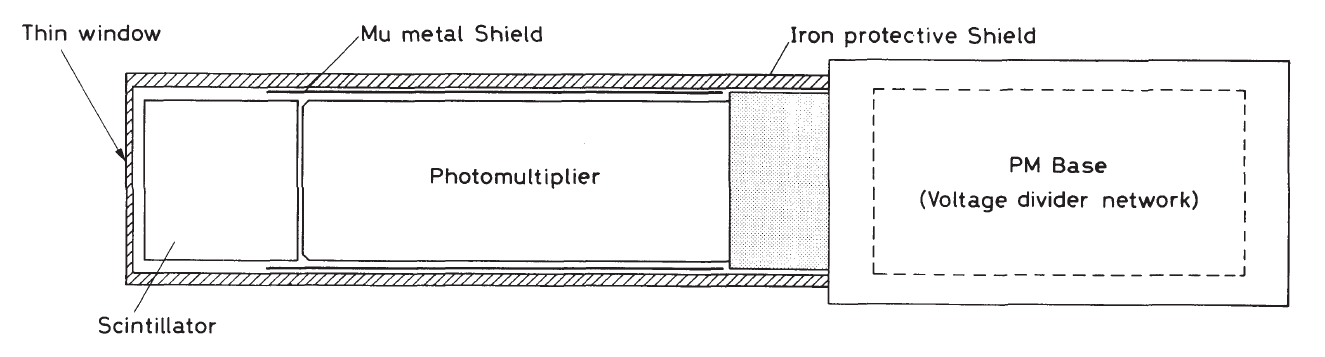
\includegraphics[width=\textwidth]{immagini/struttura_base_scintillatore.png}
\end{figure}

Ogni rivelatore basato su scintillatore prevede una parte sensibile di rivelazione, costituita da un blocco di scintillatore, che viene collegato ad un fotosensore, ossia un sensore in grado di misurare questa luce e tradurla in un segnale elettrico che poi può essere inviato in un opportuno sistema di acquisizione.

\subsection{Proprietà ideali di uno scintillatore}
\begin{itemize}[leftmargin=0.5cm]
   \item Alta efficienza di scintillazione (conversione in luce dell'energia depositata con resa fotoni/MeV elevata).\\
   Idealmente vogliamo avere un'alta efficienza di scintillazione, il che vuol dire che se una particella deposita energia, vorremmo che questa energia venisse sfruttata al meglio per produrre fotoni di scintillazione, quindi vorremmo produrre il maggior numero di fotoni in corrispondenza di una data quantità di energia depositata. Tale caratteristica viene quantificata dalla resa in luce, la quale rappresenta il numero di fotoni che vedono prodotti per ogni MeV di energia depositata;
   \item Resa in luce proporzionale all'energia depositata.\\
   Vorremmo anche che la resa in luce fosse proporzionale all'energia depositata, perché in questo modo lo scintillatore può funzionare da rivelatore che misura l'energia della particella depositata;
   \item Spettro della luce di scintillazione adatto ad essere rivelato da opportuni fotosensori.\\
   La luce prodotta dagli scintillatori viene normalmente negli UV, ma non è sempre così: a volte può essere prodotta una luce sul violetto, ma addirittura anche sul verde o sul rosso, quindi in realtà ogni materiale ha un caratteristico spettro di emissione che ha un'importanza fondamentale perché questa luce deve essere raccolta, dunque è necessario avere un sensore adatto alla luce che viene emessa, altrimenti avremmo un sistema inefficiente perché non siamo in grado di misurare questa luce. Quindi è fondamentale che lo spettro di emissione sia il più possibile vicino alla finestra di lunghezze d'onda a cui il fotosensore è sensibile, quindi bisogna individuare un accoppiamento ottimale in termini di lunghezze d'onda;
   \item Trasparenza alla luce emessa (lunghezza di assorbimento elevata).\\
   Lo scintillatore deve essere trasparente alla luce che emette. Ciò significa che la luce emessa non deve essere riassorbita, perché sennò viene persa. Ciò normalmente si realizza attraverso il drogaggio dei materiali scintillanti.\\
   In termini delle caratteristiche dello scintillatore, questo aspetto equivale a dire che la lunghezza di assorbimento deve essere elevata, dunque la luce che viene emessa deve percorrere lunghi tragitti prima di essere assorbita;
   \item Risposta veloce (tempi di decadimento piccoli).\\
   Non tutti gli scintillatori godono di questa proprietà, però ce ne sono alcuni che effettivamente hanno una risposta molto veloce e questo ci aiuta non solo per il timing, ma anche per avere delle frequenze di contenti elevate perché più è breve il segnale prima il rivelatore sarà pronto per misurare una nuova radiazione, pee cui possiamo avere anche delle frequenze di conteggio elevate;
   \item Indice di rifrazione simile a quello del vetro ($n \sim 1.5$)\\
   Ciò è legato al fatto che il rivelatore a scintillazione è sempre costituito dallo scintillatore più il fotosensore, ma non sempre le dimensioni di questi due oggetti sono comparabili, dunque non possiamo semplicemente accostarli l'un l'altro. Sorge pertanto l'esigenza di guidare la luce verso il fotosensore, quindi di creare una sorta di guida di luce che viene realizzata normalmente in plexiglass e che quindi deve avere un indice di rifrazione simile a quello dello scintillatore.
\end{itemize}

\subsection{Tipologie di scintillatori}

Come abbiamo già detto, esistono vari tipi di scintillatore, ognuno dei quali presenta una o più di queste caratteristiche. Sostanzialmente si dividono in due grandi categorie:
\begin{itemize}[leftmargin=0.5cm]
   \item Scintillatori organici, i quali sono composti da molecole contenenti atomi di carbonio, idrogeno e ossigeno. Possono essere di diverse tipologie, ad esempio potremmo avere dei cristalli organici puri, quindi dei materiali che presentano una struttura cristallina, oppure dei materiali amorfi come gli scintillatori plastici. Potremmo anche averli sotto forma di liquido, dunque si parla di liquidi organici;
   \item Scintillatori inorganici, i quali invece possono essere o dei cristalli, o scintillatori a gas o scintillatori a vetro.
\end{itemize}

\section{La luminescenza}

I materiali scintillatori presentano la proprietà nota come luminescenza. I materiali luminescenti, quando esposti a determinate forme di energia, ad esempio luce, calore, radiazioni, ecc., assorbono e riemettono l'energia sotto forma di luce visibile (o invisibile).

\subsection{Cause di luminescenza}

In generale, ci sono tanti materiali che subiscono questi fenomeni che definiamo di luminescenza, la quale si distingue a seconda del tipo di stimolo, perché per emettere della luce il materiale prima deve essere sollecitato, deve ricevere energia, e quindi a seconda della fonte di energia andiamo a distinguere diverse modalità di luminescenza. In base al tipo di stimolo con cui viene indotta la luminescenza, si parla di

\begin{itemize}[leftmargin=0.5cm]
   \item Fotoluminescenza quando il materiale viene stimolato dalla luce;
   \item Termoluminescenza se induciamo la luminescenza attraverso il calore\footnote{Un'applicazione di tale fenomeno sono le tecniche di datazione basate sulle termoluminescenze, che consistono nel far emettere materiali che hanno immagazzinato nel tempo elettroni in delle trappole i quali vengono poi liberati attraverso il riscaldamento del materiale. In base a quanta luce viene emessa si ricava il numero di elettroni che sono stati intrappolati nel tempo, deducendo così quanto tempo è trascorso e quindi si risale all'età del campione.};
   \item Sonoluminescenza attraverso un'onda sonora;
   \item Elettroluminescenza attraverso energia elettrica;
   \item Triboluminescenza attraverso deformazioni meccaniche del materiale;
   \item Chemiluminescenza attraverso reazioni chimiche;
   \item Bioluminescenza attraverso organismi viventi, tipicamente quelli che vivano a vedere nel mare, e allora si parla di bioluminescenza.
\end{itemize}

\subsection{Il processo di scintillazione}
Nel caso degli scintillatori il processo che avviene è la scintillazione, cioè emissione di fotoni a seguito di eccitazione di atomi o molecole che viene indotta da radiazione. Quindi il nostro stimolo è una radiazione che può essere una particelle o una radiazione $\gamma$. Se guardiamo in generale le caratteristiche della luce emessa per scintillazione possiamo distinguere diverse componenti:
\begin{figure}[H]
   \centering
   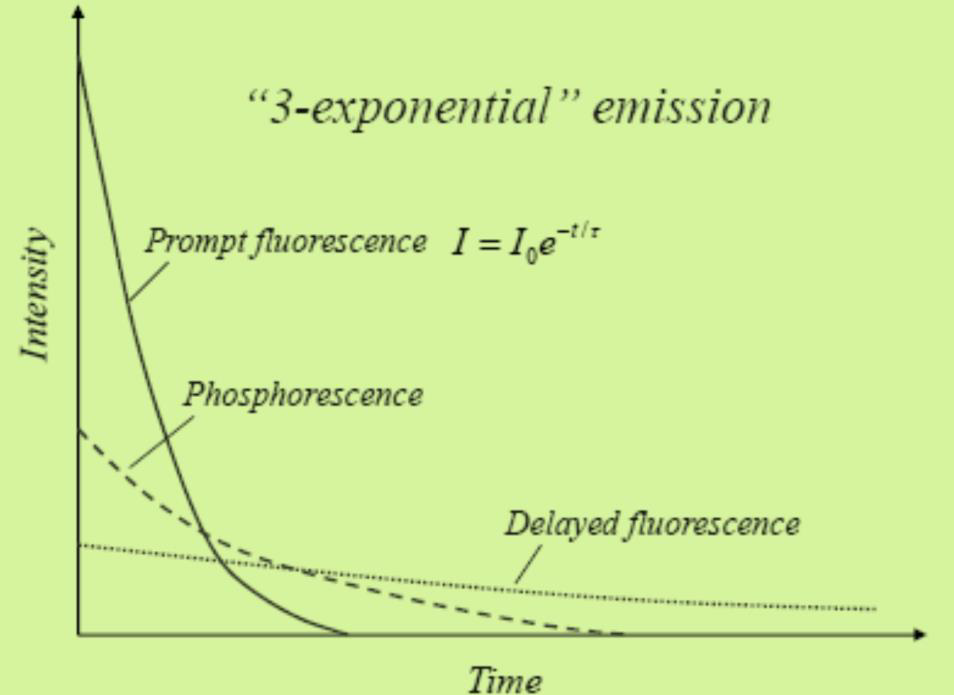
\includegraphics[width=0.6\textwidth]{immagini/tipi_di_luce.png}
\end{figure}
In generale si nota che la luce emessa diminuisce nel tempo e lo fa esponenzialmente. In altre parole, l'evoluzione nel tempo del flash di luce prodotto ha un andamento esponenziale decrescente; inoltre la pendenza di questo esponenziale dipende dalle transizioni che hanno dato luogo a questa luce.

Possiamo evidenziare diverse componenti della luce emessa:

\begin{itemize}[leftmargin=0.5cm]
   \item Abbiamo una componente prompt, cioè veloce, che è la luce di fluorescenza. Questa viene emessa con tempi caratteristici molto brevi, come dimostra la pendenza maggiore nel grafico, esaurendosi in pochi nanosecondi. Questa è la componente più veloce e anche quella più importante poiché dà il contributo maggiore potremmo;
   \item Si possono avere anche fenomeni di fosforescenza, che tipicamente sono dei fenomeni più lenti, dell'ordine dei millisecondi o secondi. Tale fenomeno è tipico dei materiali che dopo essere stati illuminati continuano a emettere luce di fosforescenza anche dopo diversi secondi\footnote{Come dice il Leo, "Se la riemissione avviene immediatamente dopo l'assorbimento o, più precisamente, entro $10^{-8} \; \rm s$ (che è all'incirca il tempo necessario per le transizioni atomiche), il processo viene solitamente chiamato fluorescenza. Tuttavia, se la riemissione è ritardata perché lo stato eccitato è metastabile, il processo è chiamato fosforescenza o luminescenza residua. In questi casi, il tempo di ritardo tra l'assorbimento e la riemissione può durare da pochi microsecondi a diverse ore, a seconda del materiale.".};
   \item Si potrebbe avere anche una fluorescenza ritardata, cioè un'emissione con dei tempi caratteristici che sono ancora maggiori, ma hanno lunghezze d'onda simili a quelle della emissione di fluorescenza.
\end{itemize}

%Ognuno di questi ha dei vantaggi e degli svantaggi, che approfondiremo nel seguito.

\section{Scintillatori organici}

\subsection{Processo di scintillazione negli scintillatori organici}

Cerchiamo di capire quali sono i principi attraverso cui abbiamo l'emissione di luce di scintillazione negli scintillatori organici.\footnote{La spiegazione dei fenomeni che portano alla produzione di luce sia negli scintillatori organici che in quelli inorganici è stata presa dal Knoll. Sebbene più approfondite, ho preferito riportare queste perché esposte in maniera più esaustiva.}

Osserviamo innanzitutto che questa luce di scintillazione è associata a transizioni di elettroni di valenza liberi, i quali sono degli elettroni che appartenono alla molecola ma non sono associati a uno specifico atomo di questa. Andiamo allora a vedere i livelli che può occupare un elettrone di questo tipo.

Una vasta categoria di scintillatori organici pratici è basata su molecole organiche con determinate proprietà di simmetria che danno origine a ciò che è noto come una struttura elettronica "$\pi$". I livelli di energia elettronici $\pi$ di una tale molecola sono illustrati nella seguente figura:
\begin{figure}[H]
   \centering
   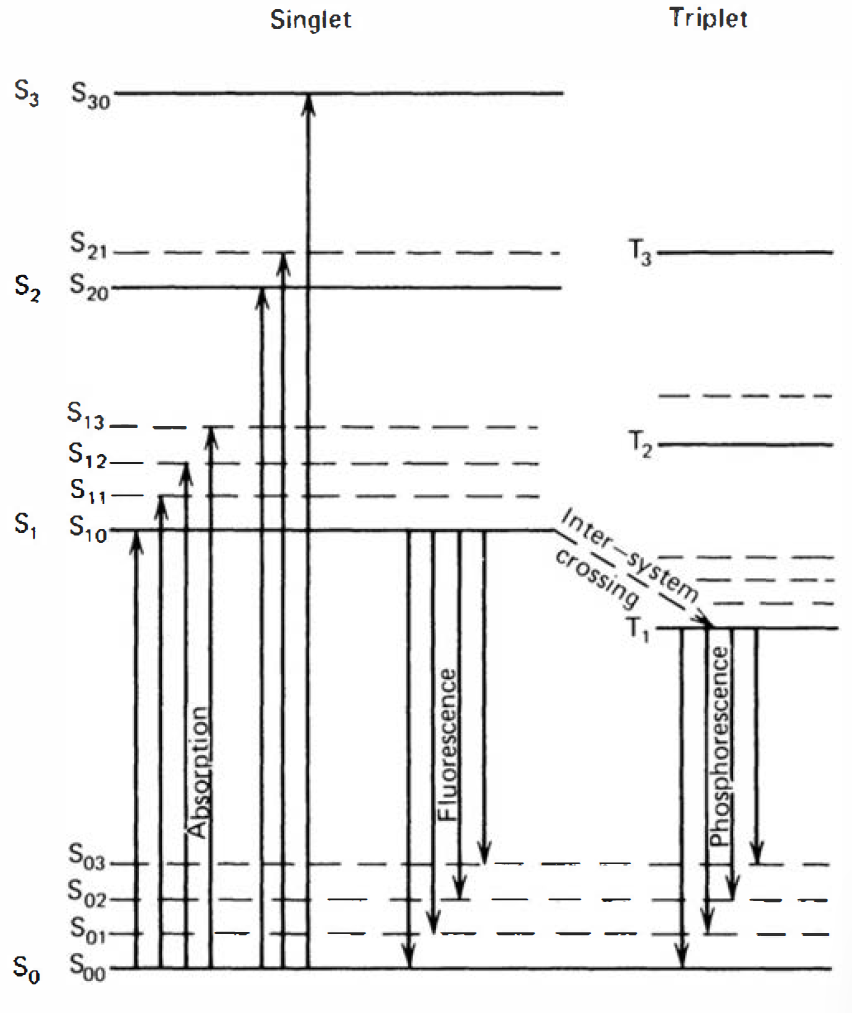
\includegraphics[width=0.7\textwidth]{immagini/Livelli_energetici_scintillatori_organici.png}
\end{figure}
L'energia può essere assorbita eccitando la configurazione elettronica in uno qualsiasi dei numerosi stati eccitati. In figura è riportata una serie di stati di singoletto (spin totale pari a 0), etichettata come $S_0, S_1, S_2, \ldots$ ed è anche mostrato un insieme di livelli elettronici detti stati di tripletto (spin totale pari a 1), etichettati come $T_1, T_2, T_3, \ldots$\footnote{Queste due tipologie di stati sono state messe una accanto all'altra soltanto per evitare di creare confusione, ovviamente ciò che conta è la loro posizione rispetto alla direzione verticale, in cui è riportata l'energia.}

Per le molecole di interesse come quelle degli scintillatori organici, il gap energetico tra $S_0$ e $S_1$ è di 3 o 4 eV, mentre lo spazio tra gli stati superiori è solitamente leggermente più piccolo. Ognuna di queste configurazioni elettroniche è ulteriormente suddivisa in una serie di livelli con spaziature molto più fini che corrispondono a vari stati vibrazionali della molecola, associati a tali moti. La spaziatura tipica di questi livelli è dell'ordine di 0,15 eV. Spesso viene aggiunto un secondo pedice per distinguere questi stati vibrazionali, e il simbolo $S_{00}$ rappresenta lo stato vibrazionale più basso dello stato elettronico fondamentale.

Poiché lo spazio tra gli stati vibrazionali è grande rispetto all'energia termica media (0,025 eV), quasi tutte le molecole a temperatura ambiente si trovano nello stato $S_{00}$. Nella figura di sopra l'assorbimento di energia da parte della molecola è rappresentato dalle frecce che puntano verso l'alto. Nel caso di uno scintillatore, questi processi rappresentano l'assorbimento di energia cinetica da una particella carica o da un $\gamma$ che passa nelle vicinanze. Gli stati elettronici di singoletto superiori, che sono stati eccitati, vengono diseccitati rapidamente (in tempi dell'ordine di picosecondi) allo stato elettronico $S_1$ tramite un processo detto di conversione interna, nel quale gli elettroni scendono verso tale stato senza produzione di radiazione. Inoltre, qualsiasi stato con un'energia vibrazionale in eccesso (come $S_{11}$ o $S_{12}$) non è in equilibrio termico con i suoi vicini e perde rapidamente quell'energia vibrazionale.

Pertanto, l'effetto netto del processo di eccitazione in un semplice cristallo organico è quello di produrre, dopo un periodo di tempo trascurabilmente breve, una popolazione di molecole eccitate nello stato $S_{10}$. La principale luce di scintillazione (o fluorescenza rapida) viene emessa nelle transizioni tra questo stato $S_{10}$ e uno degli stati vibrazionali dello stato elettronico fondamentale. Queste transizioni sono indicate in figura dalle frecce rivolte verso il basso. Se $\tau$ rappresenta il tempo di decadimento della fluorescenza per il livello $S_{10}$, allora l'intensità della fluorescenza rapida in un istante $t$ successivo all'eccitazione dovrebbe essere semplicemente
\begin{equation*}
   I=I_0 e^{-\frac{t}{\tau}}
\end{equation*}
Nella maggior parte degli scintillatori organici, $\tau$ è di pochi nanosecondi, e quindi la componente di scintillazione rapida è relativamente veloce.

La vita media del primo stato di tripletto $T_1$ è caratteristicamente molto più lunga di quella dello stato singoletto $S_1$. Attraverso una transizione chiamata "intersystem crossing", alcuni stati di singoletto eccitati possono essere convertiti in stati di tripletto. La vita media di $T_1$ può essere anche di $10^{-3}$ s, e la radiazione emessa in una diseccitazione da $T_1$ a $S_0$ è quindi un'emissione luminosa ritardata etichettata come fosforescenza. Poiché $T_1$ si trova sotto $S_1$, la lunghezza d'onda di questo spettro di fosforescenza sarà maggiore rispetto a quella dello spettro di fluorescenza. Mentre si trovano nello stato $T_1$, alcune molecole possono essere eccitate termicamente di nuovo nello stato $S_1$ e successivamente decadere tramite la fluorescenza normale. Questo processo rappresenta l'origine della fluorescenza ritardata talvolta osservata negli scintillatori organici.

\subsection{Emissione e assorbimento}

Lo schema dei livelli può essere utilizzato anche per spiegare perché gli scintillatori organici possono essere trasparenti alla propria emissione fluorescente. La lunghezza delle frecce rivolte verso l'alto corrisponde a quelle energie dei fotoni che saranno fortemente assorbite nel materiale. Poiché tutte le transizioni di fluorescenza rappresentate dalle frecce rivolte verso il basso (eccetto $S_{10}-S_{00}$, che è l'unico caso in cui la radiazione può essere riassorbita) hanno un'energia inferiore al minimo richiesto per l'eccitazione, c'è pochissima sovrapposizione tra gli spettri di assorbimento ottico e di emissione (spesso chiamata "spostamento di Stokes" o Stokes shift), e di conseguenza c'è poco auto-assorbimento della fluorescenza.

Possiamo vedere un esempio di questi spettri per uno scintillatore organico nel seguente grafico qualitativo, dove notiamo come lo spettro di emissione si trovi a lunghezze d'onda maggiori rispetto a quello in assorbimento:

\begin{minipage}{0.465\textwidth}
   \begin{figure}[H]
      \centering
      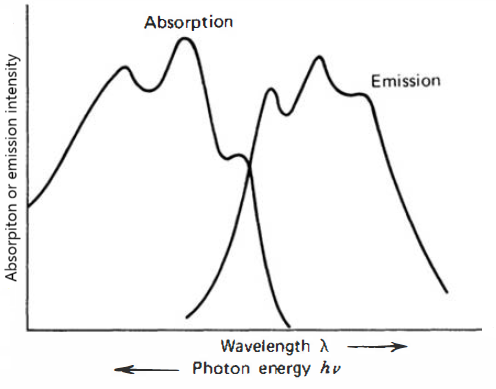
\includegraphics[width=\textwidth]{immagini/spettro_assorbimento_e_emissione_scintillatori_organici.png}
   \end{figure}
\end{minipage}
\begin{minipage}{0.53\textwidth}
   \vspace{0.3cm}Il fatto che la luce assorbita si trovi per $\lambda$ minori significa che le energie che vengono assorbite sono maggiori (in quanto $E=h\nu=\frac{c}{\lambda}$), in accordo con quanto detto prima.\\Notiamo inoltre che tra i due spettri c'è un overlap, cioè una sovrapposizione. Ciò vuol dire che la luce emessa potrebbe essere riassorbita, però nella pratica si cerca di mantenere tale overlap il più piccolo possibile.
\end{minipage}

\begin{esempio}
   Andiamo adesso a guardare uno spettro più quantitativo.
   In figura possiamo vedere lo spettro di uno scintillatore plastico:

   \begin{minipage}{0.39\textwidth}
      \begin{figure}[H]
         \centering
         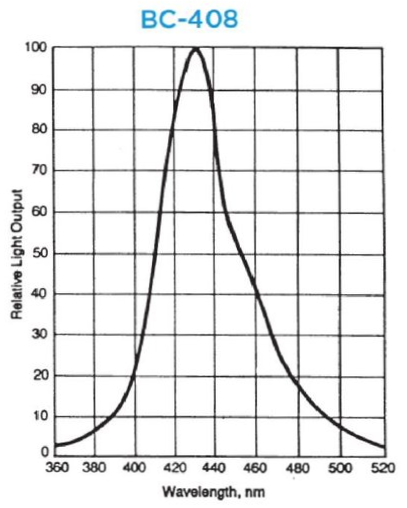
\includegraphics[width=\textwidth]{immagini/esempio_spettro_scintillatore organico.png}
      \end{figure}
   \end{minipage}
   \hfill
   \begin{minipage}{0.6\textwidth}
      \vspace{1cm}Il numero posto sopra è dovuto al fatto che, solitamente, per identificare tali scintillatori si adoperano delle sigle che derivano dalle case produttrici. 
      Guardando i valori di lunghezza d'onda notiamo che ricadiamo nella regione a cavallo tra il violetto e l'ultravioletto, addirittura la coda destra del grafico cade verso la componente azzurra. Normalmente questi spettri di emissione presentano dei picchi, per cui spesso alcuni dati che si trovano nelle tabelle (ad esempio l'indice di rifrazione del materiale, il quale dipende dalla lunghezza d'onda) si riferiscono ai valori che si hanno in corrispondenza della lunghezza d'onda del picco.
   \end{minipage}
\end{esempio}

\vfill

\section{Scintillatori inorganici}


\subsection{Meccanismo di scintillazione nei cristalli inorganici}
Mentre per gli scintillatori organici l'emissione è legata a transizioni tra livelli della molecola, in quelli inorganici il meccanismo di scintillazione dipende dagli stati energetici determinati dal reticolo cristallino del materiale.
\begin{figure}[H]
   \centering
   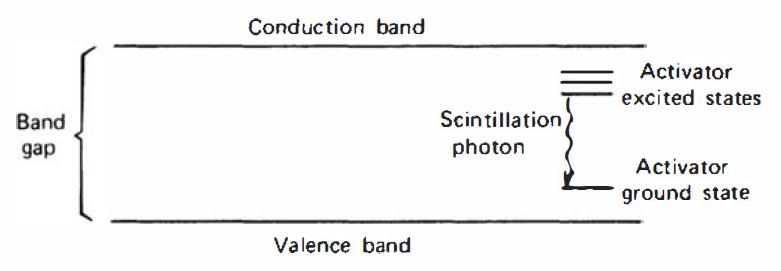
\includegraphics[width=0.75\textwidth]{immagini/Livelli_energetici_scintillatori_inorganici.png}
\end{figure}
Come mostrato nella figura sopra, gli elettroni hanno a disposizione solo bande di energia discrete nei materiali classificati come isolanti o semiconduttori. La banda inferiore, chiamata banda di valenza, rappresenta quegli elettroni che sono essenzialmente legati ai siti del reticolo, mentre la banda di conduzione rappresenta quegli elettroni che hanno sufficiente energia per essere liberi di migrare attraverso il cristallo. Esiste una banda intermedia di energie, chiamata banda proibita, nella quale gli elettroni non possono mai essere trovati nel cristallo puro.

L'assorbimento di energia può provocare la promozione di un elettrone dalla sua posizione normale nella banda di valenza oltre il gap, fino alla banda di conduzione, lasciando una lacuna nella banda di valenza normalmente piena\footnote{La professoressa afferma che si tratta di un processo ionizzazione. Tale fenomeno può essere visto in tal modo poiché implica la rimozione di un elettrone dal suo stato legato, creando una lacuna (carica positiva) e un elettrone libero nella banda di conduzione, ma è alquanto improprio perché l'elettrone non viene veramente liberato.}. Nel cristallo puro, il ritorno dell'elettrone alla banda di valenza con l'emissione di un fotone è un processo inefficiente. Inoltre, le larghezze tipiche del gap sono tali che il fotone risultante avrebbe un'energia troppo elevata per rientrare nello spettro visibile.

Per aumentare la probabilità di emissione di fotoni visibili durante il processo di diseccitazione, si aggiungono comunemente piccole quantità di impurità agli scintillatori inorganici. Queste impurità, chiamate \textit{attivatori}, creano siti speciali nel reticolo in cui la normale struttura delle bande energetiche viene modificata rispetto a quella del cristallo puro. Di conseguenza, verranno creati stati energetici all'interno del gap proibito, attraverso i quali l'elettrone può diseccitarsi ritornando alla banda di valenza. Poiché l'energia è inferiore a quella dell'intero gap proibito, questa transizione può ora dare origine a un fotone visibile e quindi costituire la base del processo di scintillazione. Questi siti di diseccitazione sono chiamati centri di luminescenza o centri di ricombinazione. La loro struttura energetica nel reticolo cristallino ospite determina lo spettro di emissione dello scintillatore.

Una particella carica che attraversa il mezzo di rivelazione formerà un gran numero di coppie elettrone-lacuna create dalla promozione degli elettroni dalla banda di valenza a quella di conduzione. La lacuna positiva si sposterà rapidamente verso il sito di un attivatore e lo ionizzerà, poiché l'energia di ionizzazione dell'impurità sarà inferiore a quella di un sito tipico del reticolo. Nel frattempo, l'elettrone è libero di migrare attraverso il cristallo e lo farà fino a incontrare un tale attivatore ionizzato. A questo punto l'elettrone può cadere nel sito dell'attivatore, creando una configurazione neutra che può avere i propri stati energetici eccitati. Questi stati sono illustrati nella figura come linee orizzontali all'interno del gap proibito. Se lo stato dell'attivatore che si forma è una configurazione eccitata con una transizione consentita verso lo stato fondamentale, la sua diseccitazione avverrà molto rapidamente e con alta probabilità di emissione di un fotone corrispondente. Se l'attivatore è scelto correttamente, questa transizione può avvenire nel campo di energia visibile (cioè si produrrà luce visibile). I tempi di vita tipici per tali stati eccitati sono dell'ordine di 30-500 ns. Poiché il tempo di migrazione per l'elettrone è molto più breve, tutte le configurazioni di impurità eccitate si formano essenzialmente allo stesso tempo e successivamente si disecciteranno con l'emivita caratteristica dello stato eccitato. È quindi il tempo di decadimento di questi stati a determinare le caratteristiche temporali della luce scintillante emessa. Alcuni scintillatori inorganici possono essere adeguatamente caratterizzati da un singolo tempo di decadimento o da un semplice esponenziale, anche se spesso si osservano comportamenti temporali più complessi.

Esistono processi che competono con quello appena descritto. Ad esempio, l'elettrone, una volta arrivato al sito dell'impurità, può creare una configurazione eccitata la cui transizione allo stato fondamentale è proibita. Tali stati richiedono quindi un incremento aggiuntivo di energia per elevarli a uno stato più elevato da cui la diseccitazione verso lo stato fondamentale è possibile. Una fonte di questa energia è l'eccitazione termica, e la componente lenta risultante della luce è chiamata fosforescenza. Spesso può essere una fonte significativa di luce di fondo o "afterglow" negli scintillatori.

Esiste una terza possibilità quando un elettrone viene catturato nel sito di un attivatore. Alcune transizioni senza radiazione sono possibili tra alcuni stati eccitati formati dalla cattura dell'elettrone e lo stato fondamentale, nel qual caso non si produce alcun fotone visibile. Tali processi sono chiamati quenching e rappresentano meccanismi di perdita nella conversione dell'energia della particella in luce di scintillazione.

In alternativa alla migrazione indipendente dell'elettrone e della lacuna descritta sopra, la coppia può invece migrare insieme in una configurazione vagamente associata, nota come eccitone\footnote{Un eccitone si forma quando un elettrone viene eccitato, ma invece di essere completamente liberato nella banda di conduzione, rimane legato a una lacuna (buco) nella banda di valenza tramite forze di Coulomb. In questo stato, l'elettrone e la lacuna formano una coppia legata. L'eccitone ha energia inferiore rispetto a quella necessaria per liberare completamente l'elettrone nella banda di conduzione, e si trova tipicamente in una banda di eccitoni appena sotto la banda di conduzione. In pratica, è una quasi-particella, una sorta di stato intermedio, dove l'elettrone e il buco si comportano come una coppia accoppiata anziché due particelle libere.}. In questo caso l'elettrone e la lacuna rimangono associati l'uno all'altra ma sono liberi di spostarsi attraverso il cristallo fino a raggiungere il sito di un atomo attivatore. Configurazioni di attivatori eccitati simili possono formarsi nuovamente e dare origine a luce di scintillazione durante la loro diseccitazione verso la configurazione fondamentale\footnote{Il processo è lo stesso del caso precedente: la lacuna strapperà un elettrone dell'atomo di impurità, solo che stavolta la lacuna non è libera bensì facente parte dell'eccitone.}.

Una conseguenza importante della luminescenza attraverso i siti degli attivatori è il fatto che il cristallo può essere trasparente alla luce di scintillazione. Nel cristallo puro, occorrerebbe approssimativamente la stessa energia per eccitare una coppia elettrone-lacuna di quella liberata quando la coppia si ricombina. Di conseguenza, gli spettri di emissione e di assorbimento si sovrapporrebbero e ci sarebbe un'assorbimento consistente da parte dello stesso materiale (self-absorption). Tuttavia, come abbiamo visto, l'emissione da un cristallo attivato avviene in un sito dell'attivatore, dove la transizione energetica è inferiore a quella rappresentata dalla creazione della coppia elettrone-lacuna. Di conseguenza, lo spettro di emissione è spostato verso lunghezze d'onda più lunghe e non sarà influenzato dalla banda di assorbimento ottico della maggior parte del cristallo.

\subsection{Spettro di emissione}

\comment{
\textbf{continua a 1:53:50 circa}

\begin{figure}[H]
   \centering
   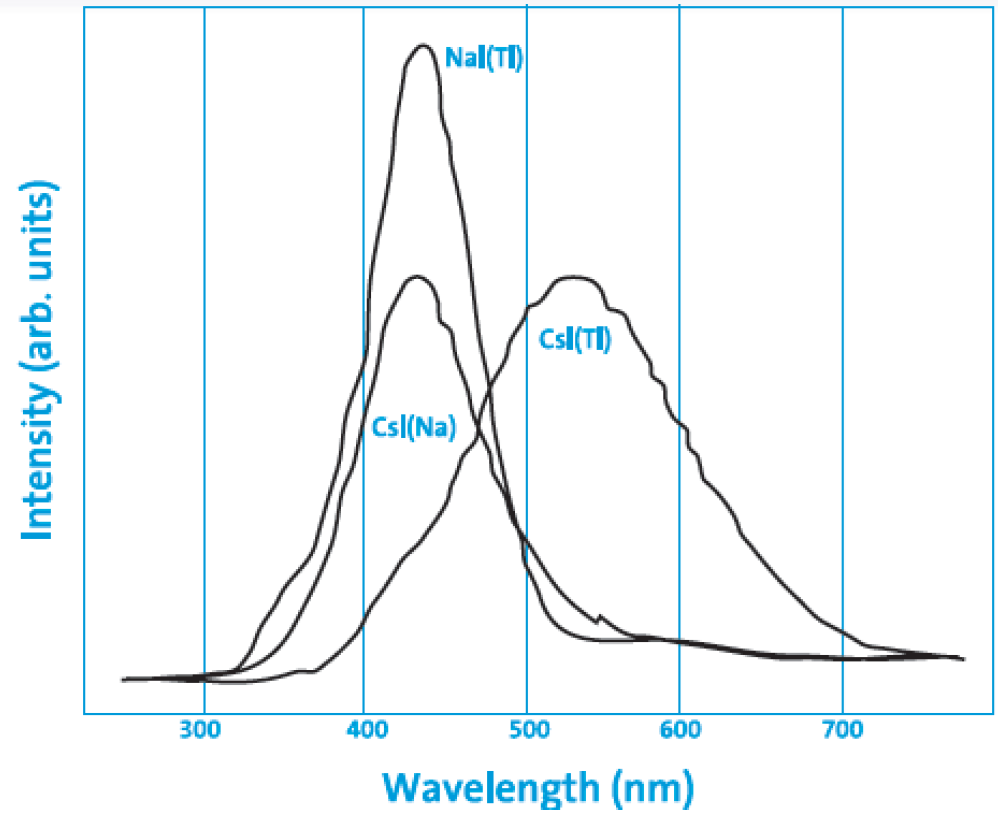
\includegraphics[width=0.6\textwidth]{immagini/spettri_emissione_scintillatori_inorganici.png}
\end{figure}

Anche in questo caso vedete dei tipici spettri che presentano un massimo e un minimo. In questo caso abbiamo gli spettri emessi da diversi scintillatori. Vedete questi sono proprio cristalli. Io duro di sodio quello che c'è trasparente, sia il materiale che vi ho utilizzato per trovare taglio. E questo è è il rivelatore che adopereremo in laboratorio. Io duro di sodio, io io che altro taglio. Ioduro di cesio, io duro la tra sodio. Ioduro di cesio, io duro la tra taglio. Quindi vedete anche in base al tipo di drogaggio, che lo cambia lo spettro di emissione, quindi cambia una caratteristica e dallo scintillatore. Non ho detto quali sono i vantaggi di questi scintillatori e vi aspetto gli scintillatori organici. Allora, gli scintillatori organici, quindi quelli composti da caracoli, ossigeno, idrogeno, hanno il bel tratto di avere una emissione molto veloce. Quindi sono dei rivelatori che vengono adoperati nel timing. Tuttavia, a causa della densità non troppo elevata, a causa del numero atomico non troppo elevato, non hanno una resa di luce particolarmente grande, perché lo stop in power è più piccolo. Quindi entro una particella, si perde energia, ma non le perde tantissimo. Viceversa, gli scintillatori inorganici hanno il vantaggio di avere una resa di luce elevata, perché hanno tipicamente delle densità notevoli, e lo vedrete, per per che hanno portato uno qui, ve lo vorrò vedere quanto è pesante uno scintillatore organico, proprio non è un classico plexiglass, si vede che è un materiale molto più denso, ha un elevato numero atomico e quindi un elevato stopping power. Questo è molto utile per la rivelazione del $\gamma$, quindi quando si vuole fare il spettroscopio in $\gamma$, dove è importante che il $\gamma$ interagisca, quindi è importante importante un elevato z o un elevato numero atomico, si utilizzano questi scintillatori. Altra faccia della medaglia, abbiamo una risposta temporale abbastanza scarsa, perché spesso i segnali sono molto lunghi, quindi questa luce viene messa anche in centinaia di nanosecondi. Altro spetto negativo è il fatto che molti materiali sono igroscopici, quindi quindi dell'umidità. E questo fa sì che devono essere riusciti a l'interno di un materiale ermetico per proteggerli dall'umidità. Vediamo alcune caratteristiche, questi sono alcuni scintillatori inorganici, quindi quelli che abbiamo visto poco fa, ioduro di sodio, ioduro di cesio, il duro di scintillatore, non entriamo nella dettaglio di tutti. Vi faccio vedere appunto, sono le caratteristiche che si vanno a vedere quando si deve scegliero uno scintillatore. Allora la densità, vedete, sono densità abbastanza elevate, partiamo dai 367 dell'ultimo di cesio, che quindi è uno dei più leggeri, possiamo dire, arriviamo a 8 per questo ton stanato di piombo o per questo liso, intorno a 7, ci sono materiali veramente molto densi. Il melting point è più un dato di interesse di chi costruisce politi. Questi scintillatori non interessano l'interesse, per esempio, la lunghezza di radiazione e il raggio di Moliere. Se vi ricordate ne abbiamo parlato, quando abbiamo descritto di sciami elettromagnetici, d'altra parte, se vogliamo misurare $\gamma$, è possibile che si sviluppi all'interno di sciami elettromagnetici, ma è importante sapere queste caratteristiche del materiale per capire quale sono le energie che posso misurare che vennero contenuti all'interno del mio rivelatore. La nutelli di interazione, c'è l'intervene di internazio per corso e che è importante, è importante, interno del micron. L'indice di rifrazione, vedete? Sono un valore molto simile al vetro, molto fondamentale. Questa è la caratteristica che finisce ombi l'impasto. Questi sono egroscopici. Ad esempio, se l'intervene di l'intervene puro di sodio, c'è una storia di un intraverso. perché incapsulata l'interno di un materiale protettivo. Allora, per luminescenza non ci interessa, ci interessa andare a guardare più che altro quest'altra caratteristica. Il tempo di decadimento, con l'unilasloppo, la pendenza, di quell'esponenziale decrescente, che ci dice quanto è stato veloce la risposta l'emissione di questa luce. E vedete, espresse in nanosecondi e abbiamo volte anche due valori che venivano riportati, perché, se mi ricordate, abbiamo detto che ci questo è una componente veloce, una componente lenta. Tante volte è soltanto la componente veloce con la che viene presa in considerazione con quella più importante, quella lenta non è quasi mai presente, comunque trascurabile. Quando viene riportata è perché effettivamente è una componente che non può essere trascurata. Lifehild è l'emissione di luce. Quanti fotomori la resa, quanti fotoni venivano prodotti per ogni mevori. In realtà qui è espressa in maniera un po' diversa, non è un numero di fotomori per me, ma si pone a 100 la resa dell'unicello di sodio, che è un materiale di riferimento, e poi rispetto a questa si esprimono tutti e altre. Quindi ad esempio il unicello di cesio emette più luce di un fattore 1,65 rispetto all'unicello di sodio. Spesso si usa anche questo modo di rappresentare questi dati. Comunque sono carnalmente resa e molto levati. In generale la resa nello scintillatore può raggiungere anche valori di 10.000 fotoni per mevori. E capite che questo ha una importanza per la risoluzione dell'energia, perché più fotoni venivano prodotti, più elevati il segnale, migliore sarà la risoluzione. Un po' come quello che abbiamo detto per i rivelatori a gas, andando a vedere il numero di coppie, il numero di cariche. Allo stesso modo di un scintillatore una risoluzione determinata da 20 fotoni venivano effettivamente emessi. Più fotoni venivano emessi, migliore sarà la risoluzione dell'energia. Quindi in generale i risoluzioni in organica hanno risoluzioni migliori. Alcuni esempi di scintillatori classici, quindi altri dati riferiti però a scintillatori classici, quindi di tipo organico, che cosa cambia rispettato prima. Vediamo i tempi di emissione, che sono molto più rapidi, nanosecondi. E poi anche qui il light ill viene riportato in percentuale rispetto all'light ill di un materiale che non trascende in questo caso specifico. Anche qui abbiamo altri valori di piccolo della lunghezza d'onda, lunghezza di attenuazione e così via. Abbiamo detto che la risposta è luce e in via di principio mi potrebbe fornire un'idea della energia depositata. Questo ovviamente se il numero di fotoni prodotto è proporzionale all'energia depositata. E questo in mezzo è vero, ma non sempre così. A volte parte dell'energia che viene depositata non viene utilizzata per produrre fotoni, viene persa attraverso dei processi non radiativi.

E questo è così che la risposta non è proprio esattamente lineare. Addirittura nel caso di particelle cariche passanti, la linearità effettivamente non è verificata. Lo vedete in questo grafico dove la resa di luce viene mostrata in funzione dell'energia. Allora intanto abbiamo una dipendenza dal tipo di particelle, quindi anche se viene depositata la stessa energia, se questa energia è depositata da un elettrone, viene messa più luce rispetto a quanta meniera è messa se l'energia viene depositata da un protone. E più vedete anche la linearità non è assicurata per le particelle cariche passanti. Quindi un grosso modo vale, ma a volte bisogna considerare delle correzioni. E proprio per quanto riguarda questa perdita di energia, esiste un modello semi-empirico che è la cosiddetta relazione di BX. Allora idealmente abbiamo detto che la resa di luce, quindi quanti fotoni vengono prodotti in base all'energia che viene depositata, dovrebbe essere una relazione lineare che lega le due grandezze, quindi se per un centimetro è stata persa una certa quantità di energia DE, allora mi aspetto proporzionalmente una quantità di luce, quindi numero di fotoni, sempre in DX. Quindi mi aspetto che se non ci sono particolari fenomeni, effetti secondari, esiste una relazione di tipo lineare. E quello che abbiamo detto prima, dove questo fattore di proporzionalità rappresenta un'efficienza massima di scintillazione. Che sostanzialmente va a stabilire la pendenza di questa curva, possiamo dire. Ma in realtà non è esattamente così che l'abbiamo capito, a volte intervengono degli effetti secondari e non radiativi degli effetti di quenching, quindi in realtà la relazione che dobbiamo prendere in considerazione è una relazione di questo tipo che però vedete tagliata a metà, quindi un attimino lo levo. Quindi rispetto a quello che abbiamo scritto prima, quindi S e DX, c'è un fattore correttivo che vedete riportato qui al denominatore, dove compare questo termine KB che è un parametro che viene ricavato da data sperimentale, come dicevo SMP, abbiamo una relazione per una parte e questa relazione viene ricavata soltanto sperimentalmente dai dati. Quindi ci aspettiamo che a causa di questi effetti non radiativi la relazione effettamente eliminale non vega sempre matta. Cosa ci aspettiamo di vedere in uscita da uno scintillatore? Il segnale che viene prodotto, capite che in realtà noi non possiamo vedere il segnale in luce, ma andiamo a vedere un segnale elettrico che viene prodotto dal fotosensore, quindi quello che si vedrà allo oscilloscopio se noi potessimo visualizzare questo segnale chiaramente è quello che produce un sensore di luce e la sua caratteristica dipendono dall'elettronico e dal tipo di sensore, quindi ad esempio più o meno ci si aspetta comunque sia una forma di questo tipo, si tratta di un segnale analogico perché a questo punto siamo interessati a quanto ha luce stata prodotta per il segnale per avere un'ampiezza proporzionale al numero di fotoni prodotti e normalmente sono segnali che hanno una durata molto breve con dei tempi di discesa di decine fino ai secondi è una durata che in realtà questa dipende un po' più dall'elettronica ma quello che ci interessa è soprattutto il fronte di salita o fronte di discesa se non ha il segnale così dimmi negativo e anche questo lo vedremo in laboratorio, quindi vedremo al oscilloscopio un tipo segnale elettriciatore allora prima di andare avanti vi faccio vedere una cosa di pratico che mi ho portato, più l'altro perché l'ho portato a non vorreste fare troppo tanto però devo ripartare una prossima volta mi stavo domando soltanto come farvele vedere più l'altro farle vedere anche a casa allora cosa vi ho portato alcune cose sono facili da farvele vedere allora questo è un esempio di scintillatore alla fine non è niente di sconvolgente perché sembra un pezzo di plexiglas sostanzialmente quindi si presenta esattamente come se fosse un plexiglas o un vetro, addirittura questo è uno scintillatore plastico quindi vedrete che la consistenza sembra quella di appunto del plexiglas più che di un vetro, un vetro più pesante di questo quindi densità non particolarmente levate quindi questi sono dei materiali che vengono adoperate molto bene per la rivelazione intanto di particelle cariche già per in $\gamma$ questi non vanno proprio benissimo perché abbiamo detto in $\gamma$ devono avere materiali più densi con alto numero atomico, ma questo invece non è così questo è stato realizzato con una tecnica di estrusione quindi con uno stampo riempito con lo scintillatore sotto forma liquida che poi viene fatta raffreddare e vedete che la superficie in questo momento è ricoperta con un materiale plastico per proteggerlo, perché comunque si ha alcuni materiali, sono sensibili anche al grasso delle mani quindi si dovranno maneggiare con i guanti la forma che è stata scelta ovviamente è stata scelta da in base allo utilizzo che dovrà fare il problema, quali sarà in questo caso andare a utilizzare un sensore in grado di misurare la luce e messa da questo 

scintillatore perché come vedremo si propaga in tutte le direzioni e quindi ora il problema sarà cercare di capire come si raccoglie la luce si deve convogliare in qualche modo in un punto della superficie perché è impensabile andare a rivestire tutta la superficie dello scintillatore con dei sensori non è realissimo, normalmente si utilizza uno, due sensori quindi bisogna convogliarle in qualche modo e poi bisogna trovare un opportuno coppimento, un opportuno sensore che divenceri deve avere quindi vi farò vedere, ora con le prossime se la idea è complesso progettare a un rivelatore che è abbastanza semplice ma in realtà bisogna cercare di ottimizzare la raccolta della luce ho lavorato tanto tempo fa con un professore che poi non l'abbiamo conosciuto del professore russo che è il papa di Marco Russo ma poi non l'abbiamo conosciuto una persona in gammo un esperimentale elettronico veramente simpatico anche e avevo lavorato su un progetto dove si utilizzavano scintillatori dove aveva raccogliere questa luce quindi dovevamo cercare di poter ottimizzare la raccolta della luce mi riconno che mi è rimasta impresso questa frase, non può volgare però proprio due due dì, rimanda tra noi lui diciava sempre, i fotoni sono bastardi perché escono è difficilissima anche una leggerissima perdita una leggerissima crepa nella copertura mi comporta delle perdite notevoli in termini di raccolta della luce quindi è un problema veramente difficile a affrontare che si deve studiare anche attraverso delle simulazioni, infatti farò vedere anche le code di simulazione per studiare il trasporto della luce per il materiale ve lo faccio girare, il mostro per farvi lo farvi vedere la seconda cosa che vi volevo far vedere sempre sui scintillatori e cercare di capire dato che sembra un pezzo di plastica come si può vedere la differenza tra un normale pezzo di plexiglass e uno scintillatore e vi racconto questo aneddoto che capitò proprio durante l'attività di produzione di alcuni fotosensori e alcuni rivelatori per l'esperimento ALICE comunque ci troviamo di fronte a un lavoro che dobbiamo fare qui a Catania dove c'era stato richiesto di realizzare delle piccole guide di luce e di accoppiarle a un sensore, dove avevamo un scintillatore una guida di luce, ora vedremo cos'è comunque lo capito dalla stessa definizione guida la luce verso il fotosensore e quindi ordiniamo queste guide di luce da una fabbrica russa o forse ucraina non mi ricordo e arrivarono queste guide di luce e arriva da certo punto un tecnico che stava lavorando con noi disse queste non sono guide di luce ma sono, quindi non sono semplici pezzi di plexiglass ma sono stati contaminati con dello scintillatore come l'ha fatto, come ha fatto a capirlo semplicemente perché ha preso uno di questi plexiglass e ha messi alla luce infatti se lo vedete l'ho alzato un po' verso la luce e poi la poi la poi un colore violetto un colore violetto, leggermente violetto e ora vi faccio vedere un effetto ovviamente questo è perché sta ricevendo la luce e la riemette sul violetto ma lo faccio vedere ancora meglio stimolando lo scintillatore con una luce che lui riesce a assorbire meglio e quindi vi ha portato qui degli senti di guide di luce che abbiamo proprio adoperato in quel periodo quindi in mezzo a questo gruppetto anzi ora hanno visto qualcuno di voi a venire e provare a fare la distinzione riconoscere così senza ovviamente metterla alla luce il plexiglass contaminato non

è un vero proprio scintillatore è messo contaminato da materiale scintillante quindi se qualcuno vuole venire a dividere è piaciuto questa sfida quindi provo a dividere in i due gruppetti quelle che tu ritieni senza guardarli vedendo risultato quelle che tu ritieni contaminato da scintillatore e quello che ritieni senza poi cosa faremo ho portato anche una lampada ovi una lampada di wood quindi poi accenderemo questa lampada e stimoleremo il materiale scintillante se è presente ok va bene questo non lo so abbiamo fatto la suddivisione ora risvegliamo tutto proviamo ad accendere la lampada di wood non so se riuscite a vederlo due ne ho persi ne ho svegliati vedi della differenza non so se riuscite se riuscite se da fuori mi viene di fare vederlo solo questi due questo è giusto quindi è riuscita abbastanza bella però si è stato imboccata quindi abbiamo un po capito che sembra apparentemente dei vedi ma in realtà sono dei materiali luminescente quindi che mettono grazie a te per la lunga scienza come appare alla fine un scintillatore montato con un fotosensore allora in questo caso vi ho portato questo altro oggetto che vedete qui questo tubo molto lungo dove in realtà il vero è proprio scintillatore e soltanto la parte argentata quindi in questo caso abbiamo un materiale scintillante di forma cilindrica è un ioduro di sodio sono sbaglio sì in questo caso è un ioduro di sodio o è quello che andrete ad operare in laboratorio quindi un scintillatore inorganico un cristallo ci aspettiamo se qualcuno vuole vederla prenderlo ne vedrà il peso sto partendo quindi ovviamente c'è anche il peso del sensore però ti rendi conto che è abbastanza pesante è molto pesante se avessi il scintillatore un paragone con il plastico vede se subito che è un materiale molto più pesante e quindi è un materiale ottimo per la rivelazione del $\gamma$ con un'alta resa che cosa c'è subito dopo c'è una guida e il sensore vero è proprio che è il foto moltiplicatore che però andremo a discutere la volta prossima non ci interessa nello specifico vi voglio far vedere soltanto che in particolare non possiamo vedere lo scintillatore perché è incapsulato con questa copertura di alluminio perché è uno dei difetti dello ioduro di sodio è il fatto di essere igroscopico e quindi bisogna necessariamente proteggerlo dall'umidità ambientale inoltre il fatto di in realtà nessuno scintillatore lo vedrete mai nudo come lo state vedendo adesso e il motivo lo spiegheremo ora quando viene prodotta questa luce quindi immaginate questo sia ad esempio una quartice ma è interno dello scintillatore e da questo punto vengono a messi i fotoni di scintillazione che abbiamo detto sono fotoni nell'uv comunque di pochi elettronVolt e questi fotoni vengono a messi in tutte le direzioni e se vengono a messi in tutte le direzioni è lasciassimo lo scintillatore nudo una ferata è chiaro che nel momento in cui i fotoni raggiungono il bordo dello scintillatore questi fuoriescono su un viscola di frazione e fuoriescono il materiale e le abbiamo persi e quindi una prima operazione che bisogna fare e cercare di evitare questi fotoni fuori escano da rivelatore secondo problema che dobbiamo affrontare l'abbiamo detto prima e cercare di convogliare i fotoni in una piccola regione dove vado a posizionare il mio fotosensore allora quello che si fa tipicamente è rivestire di un materiale possibilmente riflettente dai pareti dello scintillatore eccetto la parete dove si va la parete comunque la zona dove si va a posizionare il fotosensore ecco perché lo vedete anche coperto non soltanto per proteggerlo dall'umidità ma perché in realtà ci sarà uno strato riflettente che appunto permette alla luce di essere riflessa quindi ad esempio questo fotone che vedete qui segue queste riflessioni in questo caso stiamo vedendo una riflessione perfettamente speculare si riflette diverse volte fino ad arrivare al fotosensore capite che con uno schema del genere un fotone potrebbe anche percorrere percorsi molto lunghi prima di arrivare al fotosensore ecco perché andare a vedere la posizietta lunghezza di attenuazione è fondamentale perché è vero che magari il luce in chidatore può avere dimensioni della decina di centimetri e quindi voi possiamo dire se le lunghezze di attenuazione sono 40 cm sono tranquille, srena in realtà no perché i fotoni possono percorrere tramite queste riflessioni spazi molto lunghi quindi alla fine essere assorbiti non solo possono essere assorbiti dal materiale stesso secondo la legge esponenziale decrescente dove appunto la sloppo di questa esponenziale la pendenza è determinata da questa lunghezza di attenuazione ma potremmo avere anche effetti di assorbimento nelle pareti cioè il materiale che vado a introdurre per effettuare questa riflessione potrebbe andare ad assorbire magari non è una perfetta riflessione alcune volte sia una probabilità del 10\% di essere assorbito, il fotone non è assorbito anziché essere riflesso e quindi normalmente quando si introducono questi materiali per la riflessione si parla di coefficiente di riflettività un coefficiente che vada da 0 o 1 e che stabilisce pra un po' la probabilità di avere una riflessione o un assorbimento ad esempio un materiale che noi spesso adoperiamo ho messo qua per rivestire le pareti di uno scintillatore può essere un materiale come questo è un nastro adesivo un materiale che si chiama un nastro adesivo di miler vedete che appunto è una sorta di carta da cucina tipa alluminio come aspetto e è una superficie abbastanza riflettente quindi questa potrebbe essere una tecnica attiva, vi volevo portare anche le cuti valenti di quella mattonella di scintillatore rivestita però non l'ho trovata, non so dove è finita. Comunque in quella mattonella poi abbiamo avuto un'altra cortezza che vi schiederò a breve per andare a raccogliere la luce quindi capite che più è stesso il rivelatore più la raccolta della luce è difficile perché alla fine dei fotosensori hanno delle superfici abbastanza ridotte, non sono mai degli oggetti troppo grandi quindi più è stesso il rivelatore più abbiamo difficoltà da accoppiare il rivelatore col fotosensore quindi a fare una raccolta di luce efficiente quindi in quel caso si adoprano anche degli strategiani un po' diversi. Fino adesso abbiamo immaginato che la riflessione fosse perfettamente speculare

quindi ad esempio in un materiale del genere effettivamente mi aspetto una riflessione speculare a meno che non creo qualche rugetta nello standard il miter ma a volte si preferiscepresse utilizzare dei materiali che provocano diffusione piuttosto che riflessione quindi tificamente dei materiali o con una superficie rugosa e allora vedete la differenza. Qui abbiamo un caso di riflessione perfetta qui abbiamo un caso di diffusione. La diffusione deriva dal fatto che la superficie non è perfettamente piana e quindi quando avviene una riflessione insomma l'angolo di incidenza dipende dalla normale sostanzialmente dipende da un'inclinazione del particolare punto che viene colpito e quindi vedete uno schema molto più disordinato rispetto a una riflessione perfetta. A volte utilizziamo dei materiali diffusivi come ad esempio l'utilizzo di vernici bianche e normalmente si utilizza il biossido di ditaneo, uno di quelle vernici che vanno a rivessire il scintillatore o a volte si utilizza il teflon. Il teflon non solo l'abbiamo mai misso, viene utilizzato ad esempio nell'idraulica e quella sorta di nastro bianco si mette nelle tubature, nei raccordi per evitare le perdite. L'utilizziamo per rivessire gli scintillatori, grazie. Perché anche un materiale bianco produce diffusione e può andare bene effettivamente per il nostro scopo. Quindi dicevamo uno dei problemi che questi fotoni possono anche percorrere spazi molto grandi, lunghezze elevate e questo non solo la conseguenza di poter perdere fotoni, perché magari vengono assorbiti, ma anche conseguenze sulla risoluzione temporale, perché noi fino a adesso ci siamo concentrati sui tempi di emissione di questa luce, che abbiamo detto sono tempi molto brevi e va bene. Ma il problema è anche raccoglierla la luce a questo punto e se la luce deve percorrere spazi lunghi capite che il segnale che viene raccolto al fotosensore chiaramente può anche essere catarizzato da tempi più lunghi di quelli che abbiamo visto fino adesso. Facciamo degli esempi. Immaginate che la luce all'interno di questo scintillatore si muova a una velocità, chiaramente non è proprio la velocità della luce in quel mezzo, cioè la velocità della luce è il vuoto, ma immaginiamo che sia così, in realtà è ancora più massa. Quindi immaginiamo via U al AC e la potreste anche poi far una simulazione, ad esempio estrendo un punto a caso nello scintillatore, possiamo lavorare anche nel piano in prima approssimazione, quindi estrete un punto a caso di questa superficie dello scintillatore, estrete una direzione casuale in tutto il angolo, in tutto il duve greve, quindi 360 gradi e andate a seguire attraverso delle riflessioni il percorso di questa particella finché non arriva alla zona dove è posizionata il fotosensore e possiamo stimare quanto spazio ha percorso il fotone ed è questo sabbiliere quindi la distribuzione dei tempi, quanto tempo è impiegato a percorre quella distanza e capite che quindi idealmente se il fotone si muove se verso il fotosensore avreste tempi abbastanza brevi perché abbiamo 30 centimetri in nanosecondo, quindi se il rivelatore fosse 30 centimetri 

ci metteremo un nanosecondo a raccogliere tutta la luce, ma in realtà non è così, a seguito di queste riflessioni le distanze percorse sono molto diverse, possono essere molto diverse, abbiamo una distribuzione di distanza percorse quindi una distribuzione dei tempi per percorrere queste distanze e quindi questo rappresenta un problema soprattutto quando il rivelatore ha geometrie particolari come ad esempio nel caso di bacchette di scintillatori quindi delle barre molto lunghe con una con sezione piccola, ecco perché vi dicevo in realtà andare a ottimizzare un rivelatore di questo tipo è sempre una cosa banale, i concetti di basso sono semplici, abbiamo la produzione di luce, rifestiamo con materiale riflettente, mettiamo il fotosensore ed è fatta, in realtà purtroppo non lo voglio ridire, ma sappiamo che i fotoni non sono simpatici, bisogna ottimizzare tutto perché si rischia veramente alla fine di avere dei segnali troppo debboli, quindi di raccogliere pochi fotoni da decine di migliaia di fotoni che possono essere prodotti però ogni web alla fine se ne raccolgono qualche decina, cioè immaginate quante perdite si hanno in tutti questi processi e che cosa si può fare? Si può studiare il comportamento del rivelatore e l'arcolte di luce con dei simulatori professionali, ad esempio vi ho già parlato più volte di questo simulatore che si chiama giant di cui inesistono diverse versioni in particolare l'ultima versione giant 4 permette anche di seguire e di trasportare la luce nel materiale, nei materiali, perché la versione precedente considerava soltanto le particelle cariche, quindi i percorsi delle particelle cariche nella materia giant 4 include anche la parte dell'ottica della luce e ad esempio se voleste realizzare una simulazione, quindi seguire il percorso dei diversi fotoni che vengono prodotti per scintillazione in un rivelatore, dovreste andare a definire tantissime informazioni, ad esempio dovreste specificare che tipo di luce viene emesse per scintillazione, quindi lo spettro di emissione dello scintillatore, il tempo di decadimento, quindi quanto tempo ci si impiega a emettere questa luce, oppure si potrebbe andare a specificare l' assorbimento del materiale stesso, quindi attraverso un coefficiente di assorbimento, le proprietà di riflessione del materiale che abbiamo posto sulle pareti, effetti di rifrazione quando si passa da un mezzo a un altro, il tipo di superficie di rivestimento, se una superficie è perfettamente liscia, una superficie scabra, processi di scattering della luce e altre tipi di processi, quindi veramente è un software estremamente complesso. A titolo di esempio vi faccio vedere che si potrebbe andare a introdurre nel codice, una volta che abbiamo scelto un materiale ad esempio scelto questo materiale per andare a rivestire il mio rivelatore, vado a vedere il datasheet che mi fornisce il produttore, il costruttore di questo nastro, e scopro che il suo coefficiente, la sua riflettività cambia in base alla lombazzadonna della luce che incide, quindi non è sempre la stessa, ma cambia e ha quest'andamento, vedete, in base alla lombazzadonna, in particolare se io sono concentrata ad esempio nella riflessione di luce messa da uno scintillatore, quindi tipicamente sui 400 nanometri, vedo che addirittura in questa regione il coefficiente di riflettività varia parecchio,

quindi non è il 97\% come in questa zona ma scende anche all'83-85\% ed è importante perché cambiano tevolmente le prestazioni del rivelatore, e questi sono tutti dati che si possono passare al simulatore. Giusto per farvi vedere alcuni esempi, immaginate queste sono simulazioni che abbiamo fatto, noi a nostro gruppo di avere delle barre di lunghezza 1 metro e di sezione all'incirca 1 centimetro quadro che di voler soddare il percorso della luce all'interno di questa barra con l'idea di raccogliere la luce all'estremità, quindi la luce che viene prodotta deve percorrere anche distanze di decine di centimetri per arrivare all'estremità di vende dove è stata prodotta, di vende dove è passata la particella. E allora guardiamo quanti fotomoni riescono a percorrere una data distanza, in base alle caratteristiche del mio rivelatore, ad esempio ci sono due condizioni diverse di riflettività, 90\% 80\% e poi due condizioni diverse di superficie, se una superficie è levigata o una superficie rulosa. Allora se la superficie è posh levitata vedete che la riflettività ha un suo effetto, considerate che questa è scala logaritmica, quindi da migliaia di fotoni comunque intanto diminuisce esponenzialmente come ci aspettiamo a seguito dell'assorbimento e poi a seconda della riflettività vedete appunto che la curva blue è molto più bassa rispetto a quella rossa, in più se abbiamo una superficie scabra, appunto rivesti il rivelatore, vedete che gli effetti di riflettività ponzono di meno, ma rispetto alla superficie levigata abbiamo una notevoa diminuzione dei fotoni e questo è fondamentale, quindi ci dà delle indicazioni e non è necessario realizzare la prova sperimentale e verificare, conviene simulare prima e poi ovviamente costruire sperimentalmente. Vi dicevo che può tornare utile a volte realizzare delle guide di luce, cioè degli oggetti realizzati in plexiglass che permettano un accoppiamento più agevole tra lo scintillatore e il rivelatore, perché magari hanno proprio geometrie diverse oppure un problema che potrebbe sorgere, deriva dal fatto che magari il mio rivelatore è dentro un campo magnetico e il mio fotosensore per diversi motivi non può lavorare all'interno di un campo magnetico, perché magari sfrutta dei campi elettrici, dei moti di particelle cariche che all'interno di un campo magnetico vi conosco a molte, quindi devo portare il mio sensore fuori dal campo magnetico, come faccio a fare un accoppiamento, si possono realizzare delle guide, quindi prendere questa luce e trasportarla verso il fotosensore, capite che ognuno di questi processi, cioè ogni cosa che aggiungete comporta perdita di fotoni e lo vediamo anche qui, nel caso di una guida di luce non possiamo prendere tutti i fotoni e trasportarli su una superfice più piccola, perché in un certo senso il flusso di fotoni non è comprimibile, non valgono le stesse regole che valgono ad esempio nel trasporto dei fluidi in un condotto dove c'è ovviamente la conservazione della massa, qui al massimo possiamo trasportare una quantità di luce che è proporzionale al rapporto tra le aree, tra area del fotosensore e area dello scintillatore, non di più, quindi non possiamo pensare che tutta la luce che fuoriesce da questa superficie venga convogliata sul fotosensore che ha una superficie più piccola, al massimo possiamo convogliare questa frazione data dal rapporto delle aree, dietro questa semplice osservazione c'è ovviamente molta matematica e le guide di luce si basano sul fatto che insomma si cerca di guidare il più possibile la luce attraverso delle geometrie opportune che facilitano il fenomeno della riflessione totale. E vi dico ci sono geometrie molto varia, molto varie ad esempio questo è un classico esempio di guida di luce che si accoppia al scintillatore come questo ovvio, come questo che abbiamo visto adesso, una mattonella quindi con una sezione con una retta angolare che quindi si accoppia a questa estrenità della guida di luce e dall'altro lato invece vedete una forma cilindrica per permettere l'accoppiamento con un fotosensore che ha una superficie circolare quindi vedete questa è proprio una questione geometria e quello vedete meglio qui ad esempio scintillatore, la guida di luce e il sensore oppure vedete geometrie ancora più elaborate sono veramente delle costruzioni quasi artistiche veramente belle. Ultima cosa che vi volevo dire, mi ricordo se c'è altro, si vabbè ci fermiamo qua facciamo questo e ci fermiamo qua perché devo insegnare anche kit. Allora l'ultima cosa che vi dico è quando abbiamo una barra lunga un metro come vi ho fatto vedere prima e dobbiamo andare a raccogliere la luce dove lo posizioniamo il fotosensore, lo potrei posizionare agli estremi della barra però questo parto ovviamente prevede che la luce debba essere trasportata fino all'estremità e abbiamo visto che c'è una notevole perdita di luce a seguito di diversi effetti. Allora un'alternativa potrebbe essere quella di utilizzare le cosiddette fibre ottiche però sono fibre particolari perché si chiamano wavelength shifter fibers sono delle fibre che mi spostano la lunghezza d'onda della luce quindi assorbono la lunghezza un determinato range di lunghezza e d'onda e la riemettono a una lunghezza d'onda tipica. Ve lo faccio vedere concretamente queste sono appunto fibre di questo tipo. Vedete il colore vuol dire che emettono nel verde perché state vedendo il verde qual è la caratteristica assorbono la luce anche luce che incide lateralmente anzi lo vedete sembra quasi accese ok perché che cosa succede? Allora la normale fibre ottica e non so se abbiamo visto in altri corsi si o no? No non abbiamo mai parlato di fibre ottica? Allora la fibre ottica ha una struttura come quella che vedete qui nella slide è costituita da due cilindri concentrici allora il primo cilindro prende il nome di cor e il cuore della fibra con un determinato indice di rifrazione ed è circondato da un altro strato che prende il nome di cladding che ha un altro indice di rifrazione quindi sono due materiali con indice di rifrazione diversi in particolare l'indice di rifrazione della parte interna è maggiore rispetto a quella della parte esterna. Questo fa sì che la luce come lo vedete qui se entra con un opportuno angolazione può essere guidata attraverso la fibra ottica mediante riflessioni totali. Ricordo che la riflessione totale è permessa 

solamente se si passa da un indice di rifrazione maggiore a uno minore quindi l'idea è riuscire a guidare la luce anche in percorsi non rettiline quindi percorsi curvati attraverso queste riflessioni totali e questo è il principio di funzionamento della normale fibre ottica che viene utilizzata anche vedete lo comunicazione lo conoscete benissimo conoscete più le applicazioni che fosse il principio di funzionamento questa fibra invece la fibra webl n shifter è un po' diversa perché la fibra ottica capite può trasportare la luce solamente se la luce entra dalla sezione viene guidata ed esce dall'altro lato ok ma una luce che incide lateralmente non riesce a entrare nella fibra perché subisce pesos non è fuori ash ok questa fibra invece alla caratteristica di assorbire la luce. Quindi anche la luce che incide lateralmente viene intanto assorbita e poi riemessa alla lunghezza d'onda, in questo caso del verde. La luce che viene riemessa, siccome si trova all'interno della fibra, in automatico viene guidata verso l'esterno. Quindi capite a un funzionamento un po' diverso che a noi torna molto utile perché se io prendo questa fibra e la vado in qualche modo a distendere all'interno dello scintillatore, lei sarà in grado di assorbire la luce e messa dallo scintillatore perché la luce va a colpirare lungo tutta la sua superficie esterna, prende la luce, l'assorbe, la riemette e la guida verso l'esterno e io a quel punto posso collegare il mio fotosensore all'esterno della fibra. Come faccia incapsularla all'interno di una barra a lungo metro? Ci sono diverse tecniche, a volte con la tecnica dell'estruzione che vi ho detto prima si può realizzare una barra che presenta al centro un foro dove fa passare la fibra ottica oppure, come abbiamo fatto noi, abbiamo fatto realizzare sempre per l'estruzione una barra che presenta un solco sulla superficie. Questo solco vado a posizionare la mia fibra ottica e questa è una tecnica molto utile quando si ha a caccare con degli scintillatori di dimensioni molto estese dove diventa difficile avere fotosensori estese, quindi o si mettono tanti fotosensori e si devono far lavorare in coincidenza ma diventa complicato oppure si va a posizionar una fibra ottica e si raccoglie la luce attraverso questa fibra ottica, Wembley shifter e il fotosensore si posiziona all'estremità delle fibra ottica, più anche molto utile perché se ad esempio ho due estremità posso posizionare solamente due rivelatori, li metto in coincidenza, cioè faccio misuro solamente quando entrambi da un segnale perché se viene prodotta la luce e si incanala nella fibra ottica andrà verso il trambe l'estremità, quindi mi aspetto segnale da entrambi l'estremità e questo mi permette anche di ridurre gli eventi di rumore di fondo perché è improbabile che io abbia una coincidenza giusta appunto due segnali insieme insomma è veramente raro. Ad esempio se avessi un rivelatore molto esteso e di forma anche quadrata potrei realizzare un solco e andare a creare una spirale con una fibra ottica questo anche si fa e si va a posizionare poi un sensore da questo punto può avere anche dimensioni molto piccole, lo vedete anche del millimetro quadro e andare a raccogliere la luce con questa tecnica. Spettro di assorbimento e spettro di emissione ovviamente devono essere diversi, spettro di assorbimento si deve adattare allo scintillatore quindi deve essere verso l'UV, spettro di emissione e questo punto si deve adattare al fotosensore perché il fotosensore deve vedere questa luce. 


\textbf{lez 12}

dopo aver parlato dei rivelatori e gas abbiamo descritto quest'altra tipologia di rivelatori che sono rivelatori per certi versi più facili più maneggevoli rispetto a rivelatori a gas che comunque sia richiedono una alta tensione richiedono dei recipienti a tenuta o addirittura dei recipienti con un flusso continuo di gas gli scintillatori di per sé sono dei rivelatori a passanza basilari perché si basano se vi ricordate sulle missione di luce di scintillazione tipicamente nel UV quindi corrispondente a pochi elettron molto come energia e questa luce quindi viene messa al seguito del deposito di energia da parte di una radiazione che colpisce questo tipo di materiale e abbiamo visto anche diverse tipologie di materiale scintillatore e tipicamente l'abbiamo classificato in due grosse categorie gli scintillatori organici costituiti da composti di carbonio dirogeno sigeno e gli scintillatori inorganici l'abbiamo visto anche alcuni esempi abbiamo detto che ci sono delle proprietà caratteristiche di questi materiali che ogni volta si devono andare ad attenzionare quando si progetta un rivelatore e in particolare si può essere interessati alla resa in luce cioè il numero di fotoni che vengono emessi per ogni MeV di energia depositata perché questa chiaramente può essere un'informazione che ci dà accesso al valore di energia che è stata depositata all'interno dello scintillatore infatti tipicamente la risposta di uno scintillatore è abbastanza lineare quindi il quantitativo di fotoni che vengono emessi dovrebbe essere proporzionale all'energia depositata e chiaramente più fotoni vengono emessi migliore sarà l'efficienza scusate la risoluzione in energia del rivelatore ma anche l'efficienza perché vuol dire che quando incide una radiazione anche se viene depositata poca energia il segnale che si produce comunque un segnale che può essere rivelato e quindi aumenta anche in questo questo l'efficienza del rivelatore oltre a questo aspetto si può andare a vedere anche la risposta temporale dello scintillatore infatti abbiamo detto che in ogni scintillatore possono essere presenti due componenti una componente un po più lenta una componente un po più veloce ciò che si poto non vengono emessi tutti nell'immediato ma vengono emessi con un certo andamento nel tempo che è un andamento esponenziale decrescente che è caratterizzato tipicamente da due componenti una lente e una veloce l'abbondanza dell'une dell'altro dipende dal tipo di scintillatore che si prende in esame quindi più o meno sono queste le caratteristiche che si vanno a studiare in uno scintillatore ci sono scintillatori che magari accellono per la risposta in luce altri per la risposta temporale quindi è difficile trovare sempre lo scintillatore ideale comunque sia eravamo arrivati a discutere il fatto che questa luce una volta che viene prodotta all'interno del materiale deve essere in qualche modo guidata verso uno fotosensore perché a questo punto il problema un po come avveniva nei rivelatori angassa se vi ricordate si producevano delle 

cariche il problema era raccogliere queste cariche da luogo a un segnale elettrico a seguito della formazione di queste cariche qui il problema è è po diverso abbiamo una provizione di fotoni ma alla fine dobbiamo sempre produrre un segnale elettrico che possiamo inviare a un'opportuna elettronica e raccogliendo questi fotoni e quindi la prima cosa che si fa è cercare di convogliare i fotoni verso una porzione della superficie del rivelatore dove si posiziona un fotosensore e vi dico che appunto il fotosensore non aumenta dimensioni più piccole della superficie del rivelatore e quindi è necessario ad esempio guidare attraverso una riflessione i fotoni prodotti all'interno questo si fa se vi ricordate avvolgendo il materiale scintillatore con dei materiali riflettenti ad esempio del dei materiali simili alla carta alluminio alluminizzati oppure anche utilizzando dei materiali che provano la diffusione della luce quindi ad esempio dei nostri bianchi delle vernici bianche vanno bene lo stesso sono molto utilizzati anche in questo questo alla fine è chiaro che ogni fotone seguirà un percorso che dipende dalla punto in cui è stato emesso e dalla direzione iniziale con cui è stato emesso quindi in linea di principio anche se il percorso dal punto di emissione al fotosensore magari di pochi centimetri poche decine di centimetri in realtà se il fotone comincia a assumire delle riflessioni come in questo caso può percorrere anche distanze molto più grande rispetto a quanto previsto e questo comporta ovviamente un aspetto negativo cioè il fatto che questi fotoni possono essere persi senza essere rivelati quindi l'avevamo detto la volta scorsa ne venvano prodotti parecchi di fotoni ma in realtà soltanto una piccolissima percentuale riesce a raggiungere il fotosensore quindi per questo motivo i fotosensori che discuteremo oggi devono essere dei fotosensori intanto che sono sensibili anche a radiazioni poco intensi quindi pochi fotoni e in più devono essere anche in grado di amplificare il segnale quindi non possiamo mettere in qualsiasi fotosensore accoppiato alla scintillatora prima di andare a discutere i fotosensori volevo farvi vedere una galleria di immagini avevamo anche detto appunto che a volte gli scintillatori devono essere scintillatori devono essere accoppiati il fotosensore per questioni geometrica e quindi nasce l'esigenza di costruire delle guide di luce che sfruttano la riflessione totale dei fotoni e che convogliano che guidano la luce verso la superficie del fotosensore e avevamo concluso sono mi sbaglio la volta scorsa parlando di fibre wavelength shifter che sono appunto delle fibre che hanno preso piede nell'arco dell'ultima decina di anni e hanno il vantaggio di assorbire la radiazione che le colpisce e di riametterle e riamettere

questa radiazione verso una in una ezzadonda caratteristica della fibra quello che vi avevo portato in aula se vi ricordate era una fibra che emetteva sul verde quindi riceveva la luce che colpiva anche la superficie laterale della fibra veniva assorbita questa radiazione ad esempio vediamo qui lo spettro di assorbimento che ad esempio copre un determinato intervallo di lunghezzadonda e poi la luce viene riemessa a una lunghezza d'onda diversa shiftata spostata magari spostata verso una lunghezzadonda che va bene si accoppia bene con il sensore che noi andremo a utilizzare il fotosensore ma la cosa interessante è che appunto la luce è riemessa viene guidata all'interno della fibra verso l'estremità della fibra dove possiamo andare a posizionare un fotosensore e avevo detto che queste fibre oltre a essere molto molto cattivanti molto belle come aspetto sono molto utili quando si adoperano dei rivelatori di grandi grandi superfici quindi dei rivelatori in cui la luce viene prodotta su una superficie molto estesa e quindi bisognerà andare a ricoprire in diversi punti la superficie con dei fotosensori per essere sicuri di poter raccogliere tutta la luce prodotta e avere un'efficienza abbastanza uniforme del nostro rivelatore immaginate ad esempio di avere un rivelatore delle superfici di questo tavolo è chiaro che se io nasse ad accoppiare un solo fotosensore magari a un estremità di questo di questo tavolo è chiaro che la luce prodotta all'altra estremità potrebbe essere persa perché i fotoni dovrebbero arrivare attraverso diverse riflessioni verso il mio fotosensore quindi avrei un'efficienza non uniforme magari riesco a vedere bene le particelle che deposita una energia in prossimità del fotosensore ma tutta l'altra zona del mio rivelatore potrebbe presentare efficienza abbastanza bassa quindi ci possono essere diverse soluzioni a questo problema o utilizzare più fotosensori oppure ad esempio ad operare delle fibre web and shifter magari inserite all'interno di solchi scavati nel scintillatore per poter guidare la luce verso l'estremità della fibra dove si vanno a posizionare questi fotosensori rivelatori basati sul scintillatore vengono adoperati in diversi campi chiaramente nel campo della ricerca soprattutto fisica nucleare e astroparticellare ne vedremo alcuni esempi ad esempio per la costruzione di calorimetri vi ricordo che il calorimetro è tipicamente un rivelatore che in grado di misurare l'energia di una particella oppure rivelatori per raggi cosmici ma anche nel campo della fisica applicata vedremo anche qui alcuni esempi o applicazioni mediche qui vediamo non ve l'ho portato ma con quello vedrete poi in laboratorio un tipico esempio di un fotomoltiplicatore appoppiato una scintillatore anzi ne ho portato una volta scorso effettivamente io avevo detto appunto che lo scintillatore era solamente una porzione di quello che vedevate tutti il resto che cos'era era una guida di luce è un fotomoltiplicatore che questo caso era il fotosensore quindi tipicamente voi vedrete sempre uno scintillatore insieme un fotosensore che può essere più o meno meno a seconda del tipo di fotosensore che è stato scelto quindi in questo caso questa parte cilindrica a destra costituisce²isci lo scintillatore accoppiato a un fotomoltiplicatore che vedete sulla sinistra di cui parleremo breve chiaramente si possono anche realizzare delle strutture che comprendono più scintillatori quindi ad esempio ad esempio esempio degli array come quello mostrato in figura dove abbiamo tanti scintillatori che puntano verso una ben precisa porzione di spazio, dove magari avviene una reazione da cui vengono emesse delle particelle, quindi si realizza una corona di rivelatori, in questo caso di scintillatori, che circondano il punto di interazione analogamente. Qui vedete, siccome sono dei materiali, come vi ho detto, che possono essere lavorati facilmente, possono anche assumere delle forme caratteristiche adatte al tipo di misura che si deve effettuare. Poi ogni scintillatore ovviamente ha associato al suo fotomoltiplicatore, quindi quindi sono tantissime geometrie possibili. Oltre al campo della ricerca vi dicevo ci sono anche delle applicazioni, soprattutto in campo medico. Ad esempio gli scintillatori vengono adoperati in esami diagnostici come la PET, la Positron Emission Tomography. Quest'esame diagnostico consiste sostanzialmente nell'andare a misurare dei raggi $\gamma$ che vengono emessi da un determinato punto e vengono emessi in coincidenza, vengono emessi simultaneamente in direzione opposte. Come funziona la PET? Lo scopo, non so se abbiamo avuto un modo di fare una PET conoscete queste esame, consiste proprio nell'andare a individuare l'eventuale presenza di cellule cancerogene, che sono tipicamente delle cellule che hanno un elevato consumo di glucosio. Quindi nel paziente viene iniettato un liquido che contiene il punto del glucosio e un elemento tracciante, un isotopo che tipicamente mette dei positroni e questi positroni una volta messi si ammichilano e danno un luogo a due $\gamma$ a 180 gradi, quindi due gambe identici emessi a 180 gradi. Quindi sostanzialmente questo tracciante si concentra nelle zone all'alto metabolismo e quindi andando a ricostruire questi $\gamma$ che vengono emessi si può andare a individuare delle zone dove c'è una maggiore emissione, quindi dove si è andato a concentrare questo tracciante. E chiaramente per ricostruire due $\gamma$ a 180 gradi bisogna avvolgere in qualche modo con una corona di rivelatori il paziente e quindi in una PET si presentano delle strutture ad arco che sono costituiti da scintillatori in grado di andare a misurare questi $\gamma$. In maniera tale appunto che quando si osserva un segnale in coincidenza quindi simultaneamente un segnale in una coppia di scintillatori opposti si può andare a ricostruire quella che è la direzione di arrivo dei $\gamma$ in qualche modo quindi andando a tracciare tutti questi $\gamma$ si può andare a individuare la sorgente da cui vengono emessi questi $\gamma$. Vedete appunto lo schema della PET con questa tipica corona costituita da fotomoltiplicatori. Ora questi scintillatori fino adesso comunque nelle PET tradizionali di prima generazione erano accoppiati a fotomoltiplicatori, quindi dei fotosensori che ora andremo a vedere nel dettaglio è che avevano però lo svantaggio di non poter lavorare all'interno di campi magnetici. Vi farò vedere la struttura di un fotomoltiplicatore e capirete perché non possono lavorare all'interno di un campo magnetico quindi immaginate di voler invece sviluppare un apparato diagnostico in grado di andare a effettuare una PET all'interno di un campo magnetico perché magari si associa a una una magnetica su ogni uomo e chiaro che questo diventa limitante e per questo motivo si è pensato di andare a sostituire i fotomoltiplicatori con nuovi fotosensori di ultima generazione basati magari su materiali assatospolido quindi ci sono sassate nel corso degli anni delle evoluzioni anche di questa tecnica diagnostica e questo appunto era un tipico esempio di scintillatori di campo medico in questo caso.
}